% generated by build_assets.py from the recorded PDF and caption; do not edit
\begin{figure}[tbp]
\centering
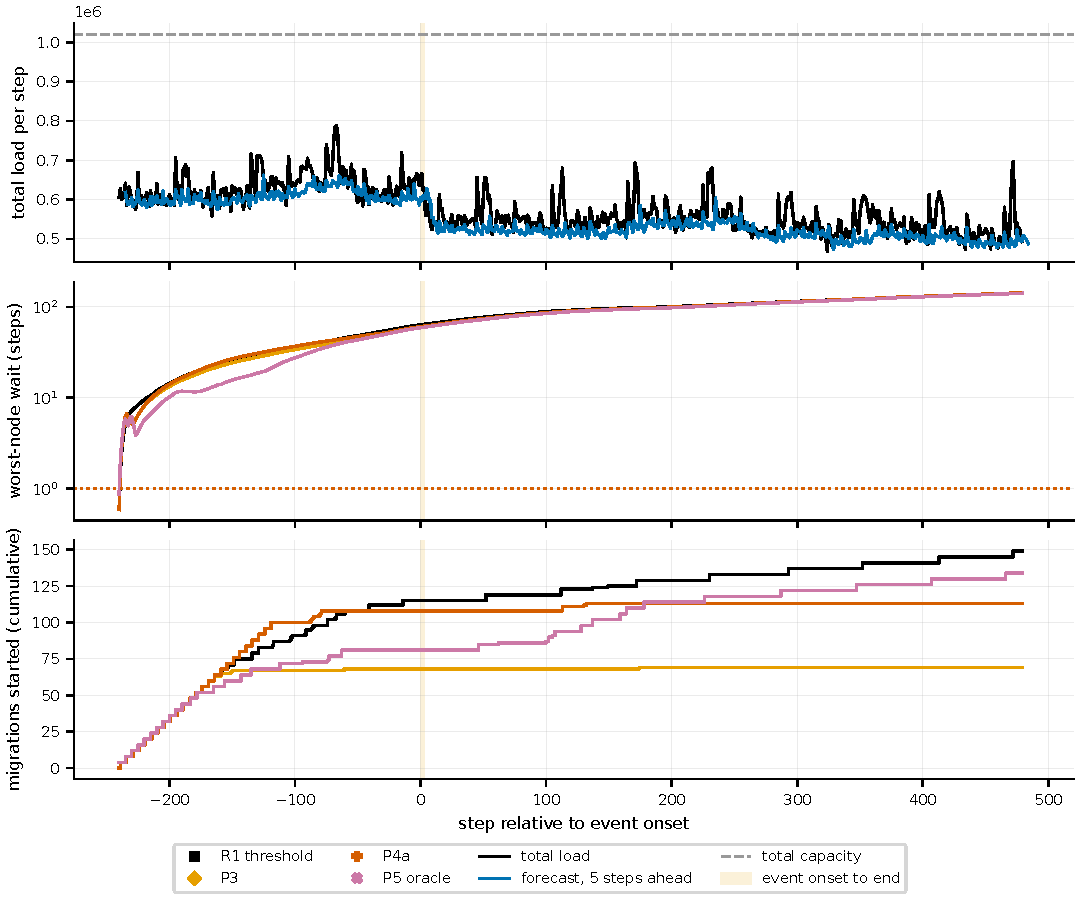
\includegraphics[width=\linewidth]{assets/figures/fa2_episode_D1.pdf}
\caption{FA2 and review Figure 3. Regenerated flash-crowd episode on D1: event D1-5320 (peak 1044), replicate 23. One replicate selected by a rule fixed beforehand, not an average, no interval. Rule: among the 30 sampled abrupt evaluation events of the default cell (m 5, headroom 1.6) the event with the median peak (lower middle on an even count, ties by event id), with the replicate index it has in the frozen rows. Top: total offered load per step, total node capacity and the point forecast of the P4 forecaster (lightgbm), summed over partitions, for the horizon of 5 steps (the default migration duration), the forecast made at step i drawn at its target step i + 5; P3 and P4a act on forecasts of this forecaster and P4a adds an interval margin that is not drawn; the shaded span runs from event onset to end. Middle: worst-node wait proxy in steps (symlog axis, SLO threshold 1 dotted). Bottom: migrations started, cumulative. Policies R1 (P1), P3 (forecaster of P4), P4a, P5. The regenerated damage and number of moves of every drawn policy equal the frozen rows (damage: R1 threshold 12.4552; P3 18.129; P4a 14.3718; P5 oracle 11.8953). Window 720 steps of 60 s, master\_seed 42. Sources: results\_frozen Must rows (P1, P3, P5) and Q1 AA6 rows (P4a), regenerated with the frozen code and configs; table of the comparison: figures/fa2\_episode\_check.csv.}\label{fig:fa2_episode_d1}
\end{figure}
